\documentclass[10pt,a4paper]{report}
\usepackage[utf8]{inputenc}
\usepackage{amsmath}
\usepackage{amsfonts}
\usepackage{amssymb}
\usepackage{graphicx}
\usepackage[frenchb]{babel}
\author{Parakian Alexis, Skrzypczak Nathan}
\title{Rubik's Cam Project PHY573a}
\begin{document}
\maketitle
\begin{abstract}
Rubik's cam est un projet développé au cours de l'Enseignement d'Approfondissement : "Conception expérimentale micro et nanoélectronique" partie FPGA. Le but étant comme son nom l'indique, d'afficher un rubik's cube à l'écran en 3 dimensions et de le résoudre à l'aide de mouvements effectués devant la caméra. Ce projet ambitieux nécessite alors la réalisation de deux parties bien distinctes qui nous permirent de se départager le travail. Nathan Skrzypczak prit en charge la réalisation d'un moteur 3D et Alexis Parakian, celle de la détection de mouvements via la caméra.
\end{abstract}

\tableofcontents
\newpage

\chapter{Présentation}

Présentation Scientifique a faire

\chapter{Architecture}

\section{Contexte et Entrées Sorties}

\subsection{Sortie VGA}

La première partie du projet à être réalisée aura été la sortie VGA. Elle l'a été sous la forme d'un composant pour plus de facilité d'utilisation. Il est contenu dans le fichier VGA\_OUT.vhd

Le point à observer en particulier est la fréquence d'horloge, en effet celle-ci conditionne la conception du reste du circuit.  On cherche à cadencer le rafraichissement à 60Hz. Une trame comprends 795 colonnes et 525 lignes (pour 640x480 utiles) soit 417900 points sur l'écran. Obtenir 60Hz par trame revient alors à \textbf{cadencer les points à 25.074Mhz}. On choisira ainsi une \textbf{fréquence utile de 25Mhz} pour rester en phase avec le reste du circuit, soit 59.82Hz par frame (on commet une erreur de 0.3\% qui est admise dans la norme VGA.
\includegraphics[width=300pt]{gfx/vga_out.png}

\begin{itemize}
\item Ce composant est cadencé sur une horloge à 25Mhz (fréquence d'affichage d'un pixel)
\item Il sort deux signaux entiers donnant la position du pixel courant :

SCREEN\_X $\left[ 0 .. 639 \right]$ et SCREEN\_Y $\left[ 0 .. 479 \right]$ sur 10 et 9 bits respectivement.
\item la couleur du pixel courant est donnée en entrée sur trois bus de 10 bits : VGA\_DATA\_R ; VGA\_DATA\_G ; VGA\_DATA\_B
\end{itemize}

\subsection{Entrées : Camera CMOS}
Concernant l'entrée par la camera, nous nous sommes inspirés d'un exemple de la bibliothèque, que nous avons quasiment entièrement réécrit. Il s'agit du programme de dialogue avec le CMOS, paramétrage de la caméra et formatage des données.

Un point particulièrement important dans l'utilisation de ce périphérique connecté au GPIO de la carte DE2 est \textbf{la gestion des horloges}. En effet, la caméra prends en entrée une horloge cadencée à 25Mhz, et retourne les données lues sur les pixels CMOS à cette même fréquence. Cependant, ce processus a une certaine durée d'exécution, surtout à cause de la présence de la nappe, et du câblage interne, qui ajoute un retard moyen de 10ns (soit $\frac{1}{4}$ de periode à 25Mhz). L'horloge générale utilisée pour le reste du circuit devra donc tenir compte de ce retard de 10ns de manière à assurer la synchronisation des données. (Voir la section Horloge pour plus de précisions)

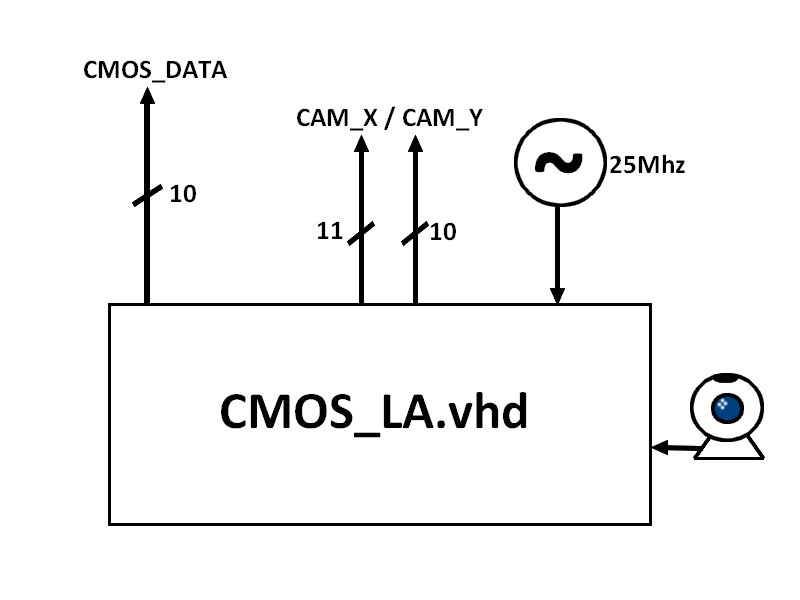
\includegraphics[width=300pt]{gfx/cmos_la.png}
\begin{itemize}
\item Ce composant est cadencé sur une horloge à 25Mhz (acquisition des pixels)
\item Il sort deux signaux entiers donnant la position du pixel courant :

CAM\_X $\left[ 0 .. (480*2-1) \right]$ et SCREEN\_Y $\left[ 0 .. (640*2-1) \right]$ sur 10 et 11 bits respectivement.
\item la couleur du pixel courant est donnée par l'organisation du capteur

\begin{center}
\begin{tabular}{|c|c|c|}
\hline 
G & R & $\ldots$ \\ 
\hline 
B & G & $\ldots$ \\ 
\hline 
$\vdots$ & $\vdots$ & $\ddots$  \\ 
\hline 
\end{tabular} 
\end{center}

\end{itemize}

\subsection{Mémoires}
Le choix des mémoires aura posé de nombreuses difficultés, dans la mesure où les composants présents fixent de nombreuses contraintes, et que le matériel disponible (pour les mémoires) possède également les siennes.
On souhaite donc afficher sur la sortie VGA une figure 3D projetée dans le plan de l'écran. Les éléments qui seront donc sujet à une forte occupation mémoire, et qui ne peuvent pas se résoudre par l'utilisation de bascules sur la carte seront donc le stockage des points de cette figure et de l'affichage de l'écran si celui-ci doit être stocké dans un buffer.

\begin{enumerate}
\item \textbf{Figure 3D}
\begin{itemize}
\item Pour la représentation en 3D de la figure, la solution la plus simple est de la décomposer en triangles (dans la mesure ou ils sont nécessairement plans). Ces triangles (ensembles de 3 points, donc 9 coordonnées de l'espace) seront tout stockés indépendamment les uns des autres par souci de simplicité. Il est possible d'optimiser grandement le stockage en utilisant des recouvrements (dans la mesure ou ils partagent souvent des sommets), mais ceci génère de la complexité dans le calcul et la gestion de cette mémoire.

\item La quantité de mémoire à prévoir pour afficher un Rubik's cube et donc en première approximation \textbf{de 108 triangles soit 972 coordonnées}. 

\item Il faut également considérer que nous manipulons des points qui seront probablement sujet à des translations et des rotations. Il nous faut donc garantir une bonne précision pour éviter la divergence des données par approximations successives. Une précision de 32bits avec virgule fixe à 16bits semble raisonnable (Avec des coordonnées allant de -32768 à 32767 et une précision de $10^{-4}$, on peut exprimer des points à 'l'infini visuel' et se prémunir des erreurs d'approximation grossières) Cette précision reste ajustable en réduisant les coordonnées accessibles. 

\item Avec ces observations, on atteint \textbf{32Kbits de données à stocker}, or le Cyclone II possède 100 puces M4K accessibles en lecture / écriture. On peut donc réaliser ce stockage directement sur la carte avec 8 telles puces.

\end{itemize}
\emph{Les triangles seront donc stockés sur une mémoire \textbf{double port} de \textbf{32bits de données} et de \textbf{10bits de bus d'adresses}.}

Les coordonnées seront stockées de cette manière pour un triangle (en partant de l'adresse 0x000) :
\begin{center}
\begin{tabular}{|c|c|c|c|c|c|c|c|c|c|c|}
\hline 
$\ldots$ & $x_1$ & $y_1$ & $z_1$ & $x_2$ & $y_2$ & $z_2$ & $x_3$ & $y_3$ & $z_3$ & $\ldots$ \\ 
\hline 
\end{tabular} 
\end{center}

\item \textbf{Ecran}
\begin{itemize}
\item Ayant vu ceci, il est nécessaire de parcourir l'ensemble des M4K occupés et de traiter les points présents pour obtenir l'image à afficher à l'écran. La fréquence d'affichage des pixels étant de 25Mhz et comme il est déraisonnable d'espérer faire fonctionner la mémoire interne à plus de 100Mhz, il est impossible de compter sur un traitement temps réel : \textbf{Nécessairement les différents pixels devront être stockés en mémoire}

\item Reste donc à définir une telle mémoire pour un écran de 640x480 pixels. La mémoire la plus simple d'utilisation offrant tout de même une capacité raisonnable est la SRAM. En effet, pour rentrer dans les 100 x M4K de la mémoire on-chip avec une profondeur de couleur de 10bits, il faudrait se limiter à 160x120...

\item La SRAM permet de stocker 256 kilomots de 16 bits ce qui est largement suffisant pour une profondeur de 10bits (niveaux de gris ou couleurs réduites) sur 640x480 pixels. Cette mémoire peut également être accédée jusqu'à 100Mhz, ce qui permet une réactivité suffisante pour la sortie VGA.

\item Pour ce qui est de la répartition des données, cette dernière est un peu subtile dans la mesure ou les plages d'adresses et de données ne sont pas paramétrables de la même façon que sur le carte. On se limite dans une première approximation à une plage de pixel de 320x240 pour simplification, mais la modification de la formule permettrait d'étendre à la résolution supérieure. L'adresse se calcule de la manière suivante:

\[ Adresse_{18bits} = \frac{x}{2} + 320 . \frac{y}{2} \]

\item On observe rapidement que le passage à 640 x 480 n'est pas particulièrement complexe, du moment que le codage des couleurs est modifié: Étant donnés les 16bits de largeur de données pour la SDRAM, on choisit un codage sur 8 bits comme suit :

\begin{center}
\begin{tabular}{|c|c|c|c|c|c|c|c|}
\hline 
R & R & R & G & G & B & B & B \\ 
\hline 
\end{tabular}
\\ Une lettre représente ici un bit - on choisit de ne stocker que les bits les plus significatifs de chaque couleur.
\end{center}

L'adresse du pixel $\left(x,y\right)$ se calcule alors par
\[ Adresse_{18bits} = \frac{y}{2}_{8bits} @ x_{10bits} \]
Avec "@" l'opérateur concaténation

On y trouve les données des pixels $\left(x,y\right)$ et $\left(x,y+1\right)$ concaténées sur la donnée de 16bits, ce qui permet de stocker l'intégralité de l'écran dans la SRAM.
\end{itemize}
\end{enumerate}

\subsection{Horloge}
Étant donné les éléments en jeu dans ce circuit, \textbf{l'horloge principale sera donc cadencé à 100Mhz} (fréquence maximale de fonctionnement de la SRAM ), de manière à permettre à cette dernière une lecture et une écriture dans une étape de calcul à 25Mhz (Une écriture dure en effet 3 cycles de 10ns et une lecture un cycle de 10ns).

La caméra induit un décalage de 10ns, on cadence donc cette dernière sur le la base 25Mhz alors que l'ensemble du circuit suit une cadence avec un cycle de 100Mhz de retard (donc 10ns)
\begin{center}
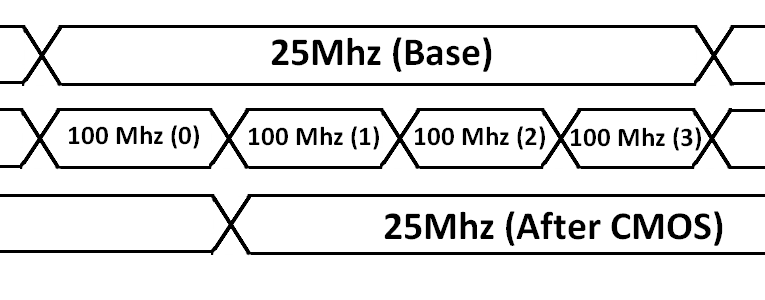
\includegraphics[width=300pt]{gfx/clock.png}
\end{center}

Ces horloges seront donc générées par un PLL du circuit:

\begin{itemize}
\item CLOCK\_50 : 50 Mhz base du FPGA
\item CLOCK\_25 : 25 Mhz PLL
\item CLOCK\_25d : 25 Mhz décalé de 10ns PLL 
\item CLOCK\_50d : 50 Mhz décalé de 10ns PLL
\end{itemize}

Le choix a beaucoup oscillé entre 100Mhz et 50Mhz pour le choix de l'horloge principale cadencent les accès SDRAM. Mais le graphe ci-dessus n'en reste pas tout autant valable.

\section{Moteur d'affichage}

C'est ce moteur d'affichage qui impose par son temps de réaction (qui ne peut pas être cadencé pour répondre en temps réel (25Mhz) à la demande des pixels) l'utilisation d'une mémoire pour l'écran et pour ses donnée personnelles.

Son fonctionnement est donc fortement dépendant de toutes ces structures de données. Il est cadencé à 25Mhz (décalé de 10ns pour suivre la Caméra) et procède par plusieurs étapes:
\begin{enumerate}
\item Les trois coordonnées constituant un point de l'espace sont dépilées et stockées dans un registre à décalage de 3x 32bits.
\item Une fois ce registre plein, la projection sur l'écran est calculée par la formule suivante:
\[ X = \frac{L}{2} + \left(x-\frac{L}{2}\right)\frac{f}{z+f} \]
\[ Y = \frac{H}{2} + \left(y-\frac{L}{2}\right)\frac{f}{z+f} \]
Où $\left(X,Y\right)$ sont les coordonnées projetées sur l'écran (de hauteur H, largeur L) ; $\left(x,y,z\right)$ les coordonnées 3D présentes dans le registre à décalage et f la focale de projection. On considère l'origine des espaces comme étant située au centre de l'écran et orientée vers l'avant comme sur la figure suivante.

\begin{center}
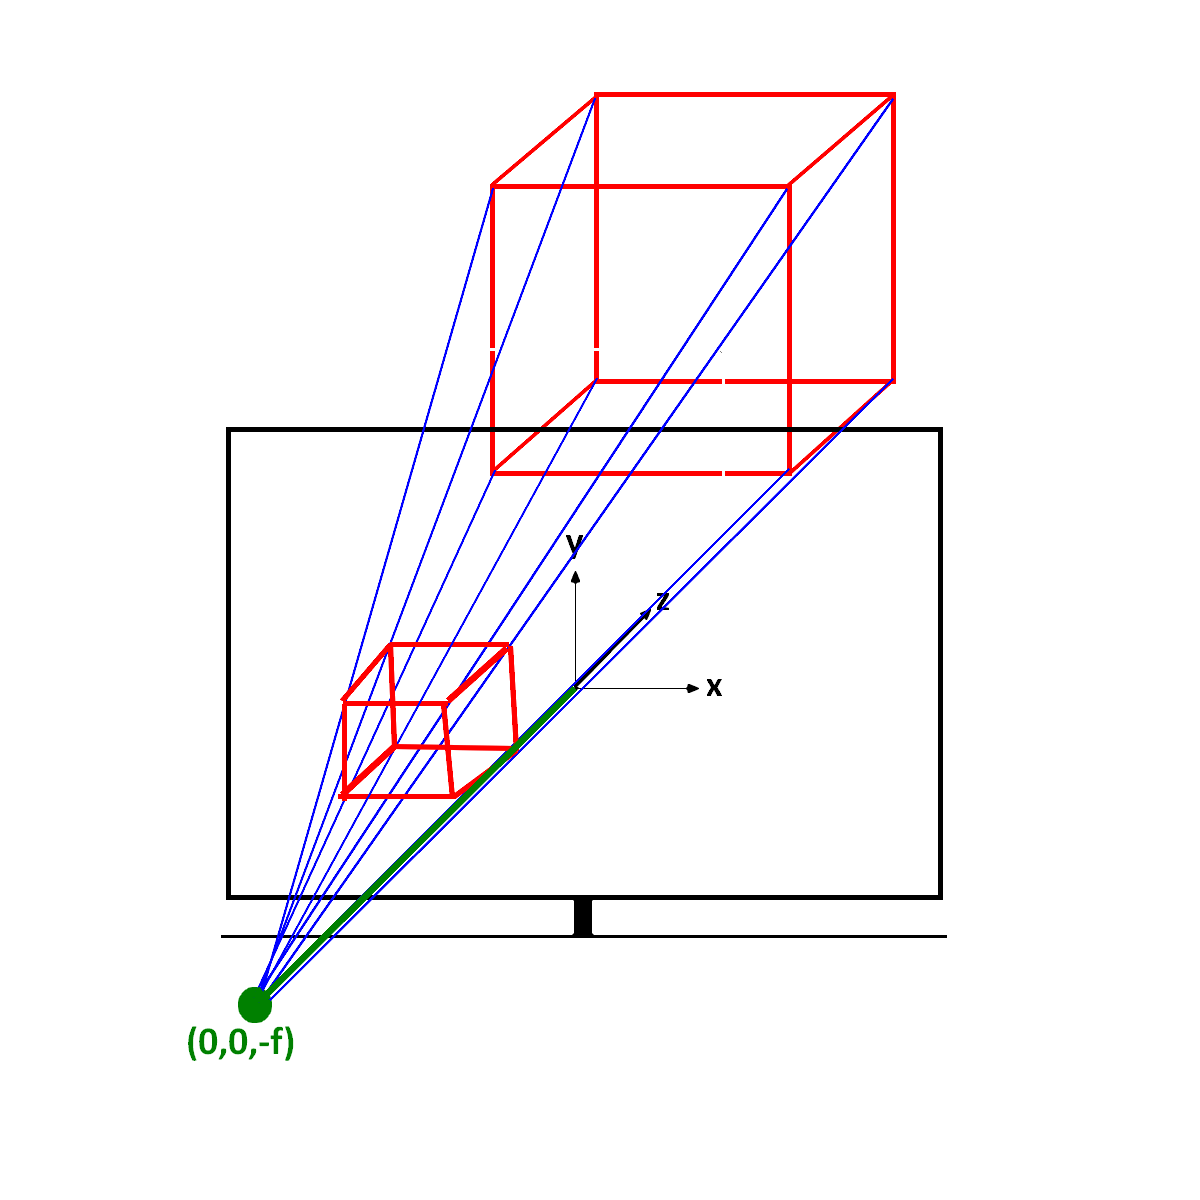
\includegraphics[width=300pt]{gfx/proj.png}
\end{center}

Projection d'ou l'on tire la formule précédente.

\item La plage mémoire associée à ces données est d'une profondeur de 32bits pour les coordonnées 3D, la virgule fixe étant définie après 16bits. Le calcul est réduit à des coordonnées entières sur 10 et 9bits (640 et 480), ce qui correspond à une troncature entière.

\item Ces coordonnées $\left(X,Y\right)$ sont ensuite à nouveau inscrites dans un registre à décalage de manière à pouvoir rassembler trois couples de coordonnées successifs afin de constituer un triangle.

\item Une fois ce triangle constitué au sein du registre à décalage, on l'inscrit dans la SDRAM - dans un premier temps en n'imprimant que les sommets - ce qui se révèle finalement le plus simple, avec la perspective de pouvoir afficher les triangles sous forme de fil de fer, puis dans un deuxième temps de les remplir (ce qui requiert alors de traiter l'occlusion d'un triangle par un autre).

\end{enumerate}

Ceci donne un composant chargé des calculs de la forme ci-dessous, avec une sortie 'couleurs' non encore définie, car dans des perspectives de test, ce composant ne sort que des points, colorés en blanc, pour ne pas surcharger la mémoire M4K et réduire la complexité du tout.
\begin{center}
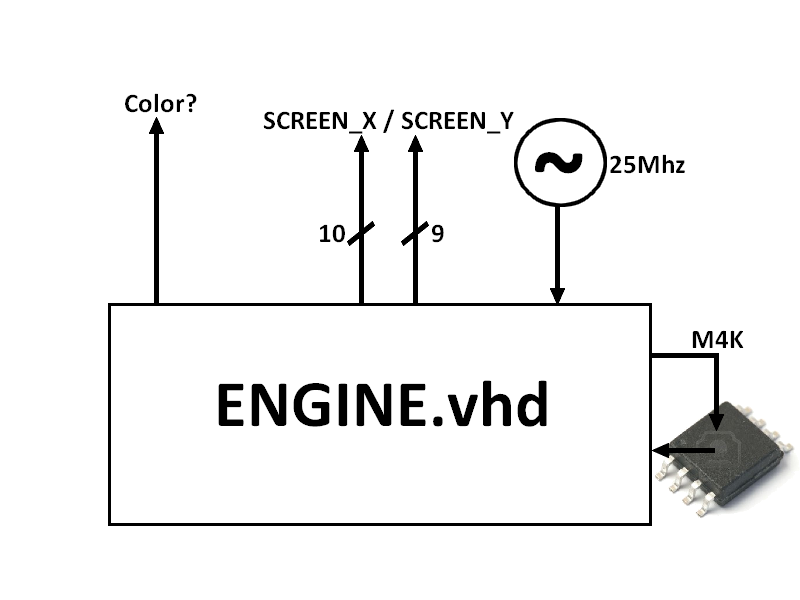
\includegraphics[width=300pt]{gfx/engine.png}
\end{center}

\section{Détection de mouvement}

Le programme de détection de mouvement est assez simpliste comparé à ce qui existe déjà mais l'idée principale était de faire quelque chose d'assez léger qui puisse tourner en temps réel et sans trop utiliser de mémoire (La SRAM et les M4K étant déjà mises à rude épreuves par le moteur 3D). 

Nous nous sommes principalement inspirés de l'algorithme de Viola et Jones de détection d'objet dans une image numérique. Cette méthode est l'une des plus connues et plus utilisées dans la détection de visages et de personnes. 

Elle consiste au parcours de l'ensemble d'une image en calculant un certain nombre de caractéristiques dans des zones rectangulaires qui se chevauchent. Pour calculer rapidement et efficacement ces caractéristiques sur une image, les auteurs proposent également une nouvelle méthode, qu'ils appellent "image intégrale. C'est une représentation sous la forme d'une image de même taille que l'image d'origine, qui en chacun de ses points contient la somme des pixels situés au-dessus de lui et à sa gauche.


Les caractéristiques sont calculées à toutes les positions (LESQUELLES?) et à toutes les échelles (LESQUELLES?) dans une fenêtre de détection de petite taille, typiquement de 24 x 24 pixels. En phase de détection, l'ensemble de l'image est parcouru en déplaçant la fenêtre de détection d'un certain pas dans le sens horizontal et vertical. Les changements d'échelle se font en modifiant successivement la taille de la fenêtre de détection. Viola et Jones utilisent un facteur multiplicatif de 1,25, jusqu'à ce que la fenêtre couvre la totalité de l'image.

Dans notre cas, nous avons du simplifier largement le programme afin qu'il corresponde aux contraintes temporelles de notre carte. En effet, les pixels de la caméra sont reçus en continus à une fréquence de 25MHz. Deux solutions s'offrent à nous.

\chapter{Connexion des blocs}

Maintenant que les différents modules du projet ont été présentés, leur agencement et leurs connexions réciproques s'effectuent de la manière suivante:

IMAGE A METTRE 

\chapter{Difficultés}

\section{Bus SRAM}
Un des problèmes principaux s'étant posé à nous au court de ce projet est la communication avec les mémoires et leur choix. Le projet était certainement trop ambitieux de ce point de vue, dans la mesure ou l'écriture sur le Bus Entrée/Sortie de la SDRAM n'a été fonctionnel que dans la dernière demi-heure de la dernière séance. Le code sous-jacent étant fondé sur des principes mathématiques relativement simplistes, il est suposé fonctionnel, mais sans la brique de la Mémoire intermédiaire pour le stockage de l'écran, il n'est malheureusement pas possible de le tester.

Le blocage du code se réalise au niveau du cadencement des lectures/écritures sur la SRAM. Dans la mesure ou l'écran impose une lecture à 25Mhz, lecture et écriture disposent chacune d'une période temporelle de 20ns pour s'effectuer. On se trouve ici particulièrement proche des valeurs minimales présentes dans la datasheet de la mémoire (de l'ordre de 15ns). De plus la commutation imposée sur le bus entrée/sortie par ce processus est également particulièrement rapide : de l'ordre de la nanoseconde entre la présence des données d'entrée et celles de sortie. C'est ce bus qui pose donc les problèmes principaux, et qui se révèlent physiquement, dans la mesure ou l'écran réplique les données qui sont écrites sur la SDRAM au moment de leur écriture: au lieu de lire le contenu de la SDRAM qui lui est addressé, l'écran se sert dans le contenu qui le moteur 3D est entrain d'inscrire sur le Bus, signe d'un mauvais cadencement de ces opérations ou d'une erreur sur la conception de ce bus.

\begin{center}
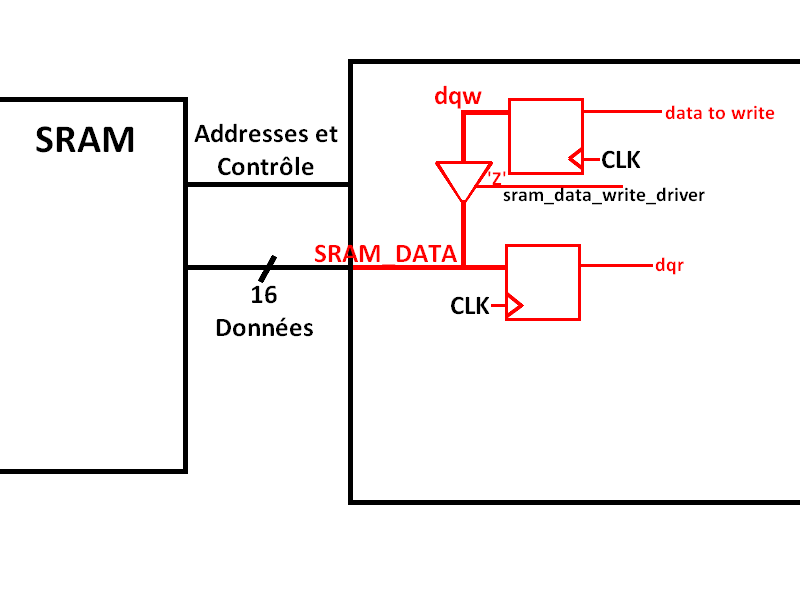
\includegraphics[width=300pt]{gfx/sram.png}
\end{center}

\section{Developpement d'un "Pong" de test}

C'est pour cette raison qu'un exemple rapide de Pong à deux joueurs à été réalisé sous la forme d'un composant annexe prenant la place de ENGINE.vhd, pour permettre d'avoir une présentation fonctionnelle dans le cas d'une incapacité à avoir une lecture / écriture correctement cadencée sur la SRAM.

Ce Pong est situé dans Pong.vhd est suit le même principe que Engine.vhd : on lui entre les signaux d'écran SCREEN\_X et SCREEN\_Y, et un signal de validité ou non du point courant (un VGA\_BLANK en somme). Il retourne alors la couleur du point courant sur 3x10bits (R,G,B). Le tout cadencé à la même fréquence que l'écran.

\begin{center}
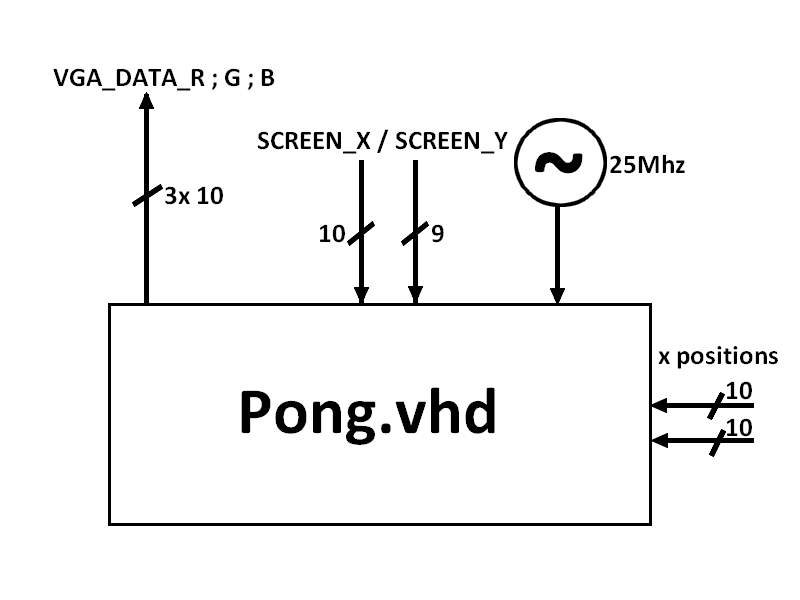
\includegraphics[width=300pt]{gfx/pong.png}
\end{center}

Ce composant réalise de simple opérations de comparaison pour obtenir la couleur du pixel courant affiché à l'écran, et garde en mémoire dans des registres locaux les informations importantes, telles que la position de la balle, celle des deux joueurs et le nombre de vies restantes. Il reste paramétrable par des entrées de position, permettant au composant d'acquisition d'influencer l'état de l'affichage et du processus en cours.

\chapter{Possibilités d'amélioration}

\section{Mémoires}

\section{Affichage}



\section{Acquisition}

On pourrait se pencher plus en profondeur sur le paramétrage fin de la caméra, et réaliser des tests voir de l'apprentissage pour que l'acquisition se fasse plus finement. Actuellement, l'exposition est réglée manuellement à l'aide de la bande d'interrupteurs de la carte DE2. On pourrait donc rechercher une valeur idéale pour ce paramètre afin de maximiser les résultats pour l'objectif nous intéressant.

\section{Reconnaissance des formes}


\end{document}